
\documentclass[10pt,journal,compsoc]{IEEEtran}

% Some very useful LaTeX packages include:
% (uncomment the ones you want to load)


% *** MISC UTILITY PACKAGES ***
%
%\usepackage{ifpdf}
% Heiko Oberdiek's ifpdf.sty is very useful if you need conditional
% compilation based on whether the output is pdf or dvi.
% usage:
% \ifpdf
%   % pdf code
% \else
%   % dvi code
% \fi
% The latest version of ifpdf.sty can be obtained from:
% http://www.ctan.org/pkg/ifpdf
% Also, note that IEEEtran.cls V1.7 and later provides a builtin
% \ifCLASSINFOpdf conditional that works the same way.
% When switching from latex to pdflatex and vice-versa, the compiler may
% have to be run twice to clear warning/error messages.






% *** CITATION PACKAGES ***
%
\ifCLASSOPTIONcompsoc
  % IEEE Computer Society needs nocompress option
  % requires cite.sty v4.0 or later (November 2003)
  \usepackage[nocompress]{cite}
\else
  % normal IEEE
  \usepackage{cite}
\fi



% *** GRAPHICS RELATED PACKAGES ***
%
\ifCLASSINFOpdf
  % \usepackage[pdftex]{graphicx}
  % declare the path(s) where your graphic files are
  % \graphicspath{{../pdf/}{../jpeg/}}
  % and their extensions so you won't have to specify these with
  % every instance of \includegraphics
  % \DeclareGraphicsExtensions{.pdf,.jpeg,.png}
\else
  % or other class option (dvipsone, dvipdf, if not using dvips). graphicx
  % will default to the controller specified in the system graphics.cfg if no
  % controller is specified.
  % \usepackage[dvips]{graphicx}
  % declare the path(s) where your graphic files are
  % \graphicspath{{../eps/}}
  % and their extensions so you won't have to specify these with
  % every instance of \includegraphics
  % \DeclareGraphicsExtensions{.eps}
\fi

% *** ALIGNMENT PACKAGES ***
%
%\usepackage{array}

% *** SUBFIGURE PACKAGES ***
%\ifCLASSOPTIONcompsoc
%  \usepackage[caption=false,font=footnotesize,labelfont=sf,textfont=sf]{subfig}
%\else
%  \usepackage[caption=false,font=footnotesize]{subfig}
%\fi





% *** Do not adjust lengths that control margins, column widths, etc. ***
% *** Do not use packages that alter fonts (such as pslatex).         ***
% There should be no need to do such things with IEEEtran.cls V1.6 and later.
% (Unless specifically asked to do so by the journal or conference you plan
% to submit to, of course. )
\usepackage{cite}
\usepackage{amsmath,amssymb,amsfonts}
\usepackage{algorithmic}
\usepackage{graphicx}
\usepackage{textcomp}
\usepackage{url}

% correct bad hyphenation here
\hyphenation{op-tical net-works semi-conduc-tor}


\begin{document}
%
% paper title
% Titles are generally capitalized except for words such as a, an, and, as,
% at, but, by, for, in, nor, of, on, or, the, to and up, which are usually
% not capitalized unless they are the first or last word of the title.
% Linebreaks \\ can be used within to get better formatting as desired.
% Do not put math or special symbols in the title.
	%\title{Bare Demo of IEEEtran.cls for\\ IEEE Computer Society Journals}
%
\title{Overtaking Uncertainty with Evolutionary TORCS controllers: Combining BLX-$\alpha$ Operator and Grand Prix Selection}

\author{Mohammed~Salem, Antonio~M.~Mora, and~Juan~J.~Merelo% <-this % stops a space
\IEEEcompsocitemizethanks{\IEEEcompsocthanksitem M. Salem was with the Department of Computer Sciences, University of Mascara, Algeria.\protect\\
% note need leading \protect in front of \\ to get a newline within \thanks as
% \\ is fragile and will error, could use \hfil\break instead.
E-mail: salem@univ-mascara.dz
\IEEEcompsocthanksitem A~M.~Mora was with the Department of Signal Theory, Telematics and Communications, ETSIIT-CITIC, University of Granada, Spain.\protect\\
Email: amorag@ugr.es
\IEEEcompsocthanksitem J~J.~Merelo was with the Department of Computer Architecture and Computer Technology. University of Granada, Spain.\protect\\
Email: jmerelo@geneura.ugr.es
}% <-this % stops an unwanted space
\thanks{Manuscript received December XX, 2019; revised XXXX, 2020.}}

% note the % following the last \IEEEmembership and also \thanks - 
% these prevent an unwanted space from occurring between the last author name
% and the end of the author line. i.e., if you had this:
% 
% \author{....lastname \thanks{...} \thanks{...} }
%                     ^------------^------------^----Do not want these spaces!
%
% a space would be appended to the last name and could cause every name on that
% line to be shifted left slightly. This is one of those "LaTeX things". For
% instance, "\textbf{A} \textbf{B}" will typeset as "A B" not "AB". To get
% "AB" then you have to do: "\textbf{A}\textbf{B}"
% \thanks is no different in this regard, so shield the last } of each \thanks
% that ends a line with a % and do not let a space in before the next \thanks.
% Spaces after \IEEEmembership other than the last one are OK (and needed) as
% you are supposed to have spaces between the names. For what it is worth,
% this is a minor point as most people would not even notice if the said evil
% space somehow managed to creep in.



% The paper headers
%\markboth{Journal of \LaTeX\ Class Files,~Vol.~14, No.~8, August~2015}%
%{Shell \MakeLowercase{\textit{et al.}}: Bare Demo of IEEEtran.cls for Computer Society Journals}
% The only time the second header will appear is for the odd numbered pages
% after the title page when using the twoside option.
% 
% *** Note that you probably will NOT want to include the author's ***
% *** name in the headers of peer review papers.                   ***
% You can use \ifCLASSOPTIONpeerreview for conditional compilation here if
% you desire.



\IEEEtitleabstractindextext{%
  \begin{abstract}
    Evolution is a powerful problem-solving technique, and it has been
    extensively used for designing racing car controllers. It present
    a series of challenges: it needs an evaluation function that is
    able to separate the best controllers from the rest, and it needs
    a series of operators that are able to explore many different
    possibilities in the controller search space. But racing scores
    are variable and also depend on adversaries and the actual track,
    and this uncertainty also means that it is much more important to
    maintain a high diversity. Building on the experience drawn from
    our previous work, in this paper we evaluate a kind of fitnessless
    selection based on competition and called Grand Prix Selection (GPS), which should be able to reduce uncertainty by using something more realistic than solo race scores to select individuals; however, uncertainty has the
    unintended side effect of increasing diversity, so we will
    evaluate the diversity-increasing BLX-$alpha$ operator in
    combination with them, and see its effects on overall
    performance. In general, results will show that these combined
    improvements establish a new level of performance of evolved
    controllers, being able to beat, both standard and previously evolved controllers, as well as a high-ranked controller of TORCS competitions.
\end{abstract}

% Note that keywords are not normally used for peerreview papers.
\begin{IEEEkeywords}
Simulated Car Racing, TORCS, Fuzzy Controllers, Autonomous controllers, Genetic Algorithms, Optimization, BLX-$\alpha$ Crossover, Grand Prix Selection, Uncertainty
\end{IEEEkeywords}}

% make the title area
\maketitle


% To allow for easy dual compilation without having to reenter the
% abstract/keywords data, the \IEEEtitleabstractindextext text will
% not be used in maketitle, but will appear (i.e., to be "transported")
% here as \IEEEdisplaynontitleabstractindextext when the compsoc 
% or transmag modes are not selected <OR> if conference mode is selected 
% - because all conference papers position the abstract like regular
% papers do.
\IEEEdisplaynontitleabstractindextext
% \IEEEdisplaynontitleabstractindextext has no effect when using
% compsoc or transmag under a non-conference mode.



% For peer review papers, you can put extra information on the cover
% page as needed:
% \ifCLASSOPTIONpeerreview
% \begin{center} \bfseries EDICS Category: 3-BBND \end{center}
% \fi
%
% For peerreview papers, this IEEEtran command inserts a page break and
% creates the second title. It will be ignored for other modes.
\IEEEpeerreviewmaketitle



\IEEEraisesectionheading{\section{Introduction}\label{sec:introduction}}

% Antonio - Is somebody writing this? I guess it is incomplete (something is missing before)... :_D

In a simulated and
    realistic racing car environment, however, racing car scores are a
    statistical variable whose value will vary depending on track and
    (simulated) atmospheric conditions; and we should never forget
    that score in a training track will always be a surrogate of its
    actual score when racing against other cars in different tracks,
    which adds another layer of uncertainty.


% The two new techniques introduced in this paper, namely, \textit{Grand Prix selection} (GPS) and $BLX-\alpha$ crossover, try to improve on previous results by first relying less on the surrogacy of the fitness function
% to select the best individuals. The GPS will use a parameter-less fitness function to select a few individuals that will race against each other; racing will {\em smooth out} randomness in the fitness by putting them in a
% more real environment; racing cars against each other will offer a
% result that varies much less than simply comparing fitness. But, even
% so, uncertainty is present in the fitness and we should avoid
% excessive exploitation of the results. The $BLX-\alpha$ crossover we
% have introduced takes care of this aspect.


The algorithm proposed in this paper overcomes most of the problems we
have found in this line of research, that started with
\cite{DBLP:conf/evoW/SalemMMG17}, which was a basic system that
introduced fuzzy controllers for driving the car and continued with
\cite{10.1007/978-3-319-77538-8_24}, where the shape and values of the
fuzzy controllers were improved using an evolutionary algorithm; that
algorithm was improved in \cite{DBLP:conf/ipmu/SalemMGG18}. However,
we still had to deal with uncertainty, as well as a not so good
exploration of the parameter space; the issue that we were using a
surrogate of the real bot capacity by doing solo races was tackled by
trying to use different fitness functions, but also by racing the best
individuals in the last generation, which we introduced in
\cite{salem_cig2018}. Introducing races in the selection of the
``winner'', even if it was in the last generation, improved results,
so this kind of competitive selection was extended by introducing real
races from every few generations in 
\cite{DBLP:conf/cig/SalemMG19} we introduced the BLX-$alpha$. The
results were the best obtained so far, so in this paper we are testing
a kind of fitness-less selection, which we call Grand Prix, combined
with others or by itself, as the only way for car controllers to be
selected for the next generation.

%The rest of the paper is organized as follows. Next we present the
%state of the art, to be followed by a description of the TORCS
%simulator \ref{sec:torcs}, the defined fuzzy controllers \ref{sec:subcontrollers} and a deep explanation of the Genetic Algorithm implemented and tested in this work in Section \ref{sec:GA_optimization}. 
%After it, the experiments conducted and the obtained results are described in Section \ref{sec:results}. Finally, conclusions and future lines of work will be presented in Section \ref{sec:conclusions}.


%%%%%%%%%%%%%%%%%%%%%%%%%%%%%%  STATE OF THE ART  %%%%%%%%%%%%%%%%%%%%%%%%%%%%%%
\section{State of the Art}
\label{sec:soa}


% We have to focus the state of the art in three different things
% 1. First and foremost, uncertainty in evolution, since it's in the
% title of the paper.
% 2. Second, alternative selection operators used in games, similar to
% the Grand Prix selection.
% 3. State of the art in TORCS since our last paper (CoG 2019)

% \cite{loiacono2010learning} cites for the first time reinforcement
% learning. Still one of the most popular methods, like
% \cite{giani2019desing,remondaformula,waghdistributed}; in the last
% case, the method is called asynchronous advantage actor-critic
% reinforcement algorithm.

% \cite{vrajitoru2019trajectory,vrajitorugenetic} maps the trajectory using the first lap and then optimizes it using an evolutionary algorithm.
% \cite{mirus2019short} uses neuromorphic architecture, namely,
% spiking neural networks. Choses one training, one validation track
% only. Tracks "that show similar characteristics in road width and
% occurring curvatures." Uses CGTrack 2 for training

% \cite{8833873} uses CG Track 2 and "deep learning", working with
% real images instead of sensors.

% \cite{10.1371/journal.pone.0213193} uses neuroevolution, and also
% CG-TRACK1

% \cite{Kole-ParamCarTunning12} mentions CG-Track 2 is "relatively
% harder", with E-Track 3 the hardest,
% \cite{verma2018programmatically} uses CG-Track 2 as a test track for
% transfer learning.


%%%%%%%%%%%%%%%%%%%%%%%%%%%%%% TORCS  %%%%%%%%%%%%%%%%%%%%%%%%%%%%%%

The TORCS racing simulator continues to be one of the main platforms
for testing different autonomous driving or bot creation strategies,
which are, by and themselves, also a hot topic in the gaming arena as
well as by itself, at least since DARPA created their autonomous car
challenge \cite{badue2019selfdriving};
only in the last year (2019) there are around 200 articles that
mention it; during  \cite{schiavullo2019torcs} of its
applications for the last 20 years; they are but one of the possible
platforms that are used for this kind of problem; a good review
(focused on reinforcement learning) was made by
\cite{abuzekry2comparative}. Fuzzy controllers are mentioned in around
15\% of them, while around 30\% mention evolutionary algorithms; very
few, however, around 7\%, use both, and most of them are not actually
using TORCS.

There are several possible approaches to autonomous driving and its
solution using TORCS: you can use vision to have more complete,
although more complicated, view of where the car is and where it's
going, or just use sensors, which only check the most immediate
scenario, but on the other hand are more precise and easy to check; in
our case, we have opted for the latter, although other papers like the,
ones authored by Zhu et al. \cite{zhu2018driving,zhu2019vision,neurone} rather
use vision, using TORCS as a testbed for a different kind of algorithms.


% Fitlessness coevolution: playing games to select, defined in
% \cite{Jaskowski:2008:FC:1389095.1389161}. This is a precedent to our
% "grand prix" selection. That article cites
% \cite{Angeline:1993:CEE:645513.657590} as the first reference,
% calling it "competitive fitness environment", and later developed in
% \cite{rosin1995methods}, but it's been also used in GP by Tettamanzi
% in \cite{tettamanzi1996genetic}. First time used in
% games in \cite{luke1998genetic}, but later used extensively, like
% \cite{Jaśkowski2008,10.1007/978-3-540-78671-9_2,alhejali2011using}. As recently as 2017, an ELO-based ranking
% strategy was introduced for selecting winning bots in a fighting
% game \cite{7792145}. The first one mentions "imperfect information"
% as one of the factors to use this fitlessness strategy.

\section{The Open Racing Car Simulator}
\label{sec:torcs}

The framework in which this study has been conducted is TORCS \cite{torcs4}. It is an open source, multi-player, modular and portable racing simulator that allows users to compete against other computer-controlled opponents.
Its high degree of modularity and portability, together with the
realistic and real-time driving simulation, make it an ideal testbed
for artificial intelligence research, as stated in previous section.

Every car in TORCS includes  a large set of sensors \cite{manualTORCS},
whose values the car can use during a race, such as distances to track borders, to rivals, current fuel, current gear, position in the race, speed, or damage, among others. See Figure \ref{fig:torcs-sensors}.

\begin{figure}[!ht] 
	\begin{center}
		\includegraphics[scale=0.35]{fig/torcs-sensors}
		\caption {TORCS capture showing some of the sensors that the car includes.}
		\label{fig:torcs-sensors}
	\end{center}
	% Antonio - if we need space we can remove this image
\end{figure}


The sensor values are considered by any TORCS autonomous controller, or
{\em controller}, to manage the car using actuators \cite{manualTORCS}: the
steering wheel, the accelerator, the brake pedal and the gearbox.   


%*****************************  FUZZY CONTROLLER  ******************************

\section{Fuzzy sub-controllers}
\label{sec:subcontrollers}



%%%%%%%%%%%%%%%%%%%%%%%%%%%%  OPTIMISING WITH GAS  %%%%%%%%%%%%%%%%%%%%%%%%%%%%

\section{Evolutionary Algorithm}
\label{sec:GA_optimization}

% ----------------------------- We need to rewrite most of this
% ---------------
% Antonio - done. I have rewritten it
% No, you haven't. It's still pretty much the same. Marked paragraphs
% that are taken from the other paper - JJ

As aforementioned, the proposed fuzzy sub-controllers were optimised by means of a Genetic Algorithm (GAs) \cite{GAs_Goldberg89}, aiming to find the optimal parameter values of their respective membership functions.

The followed process is shown in Figure \ref{fig:ga}. 

 \begin{figure}[!ht]
 	\label{fig:ga}
 	\begin{center}
 		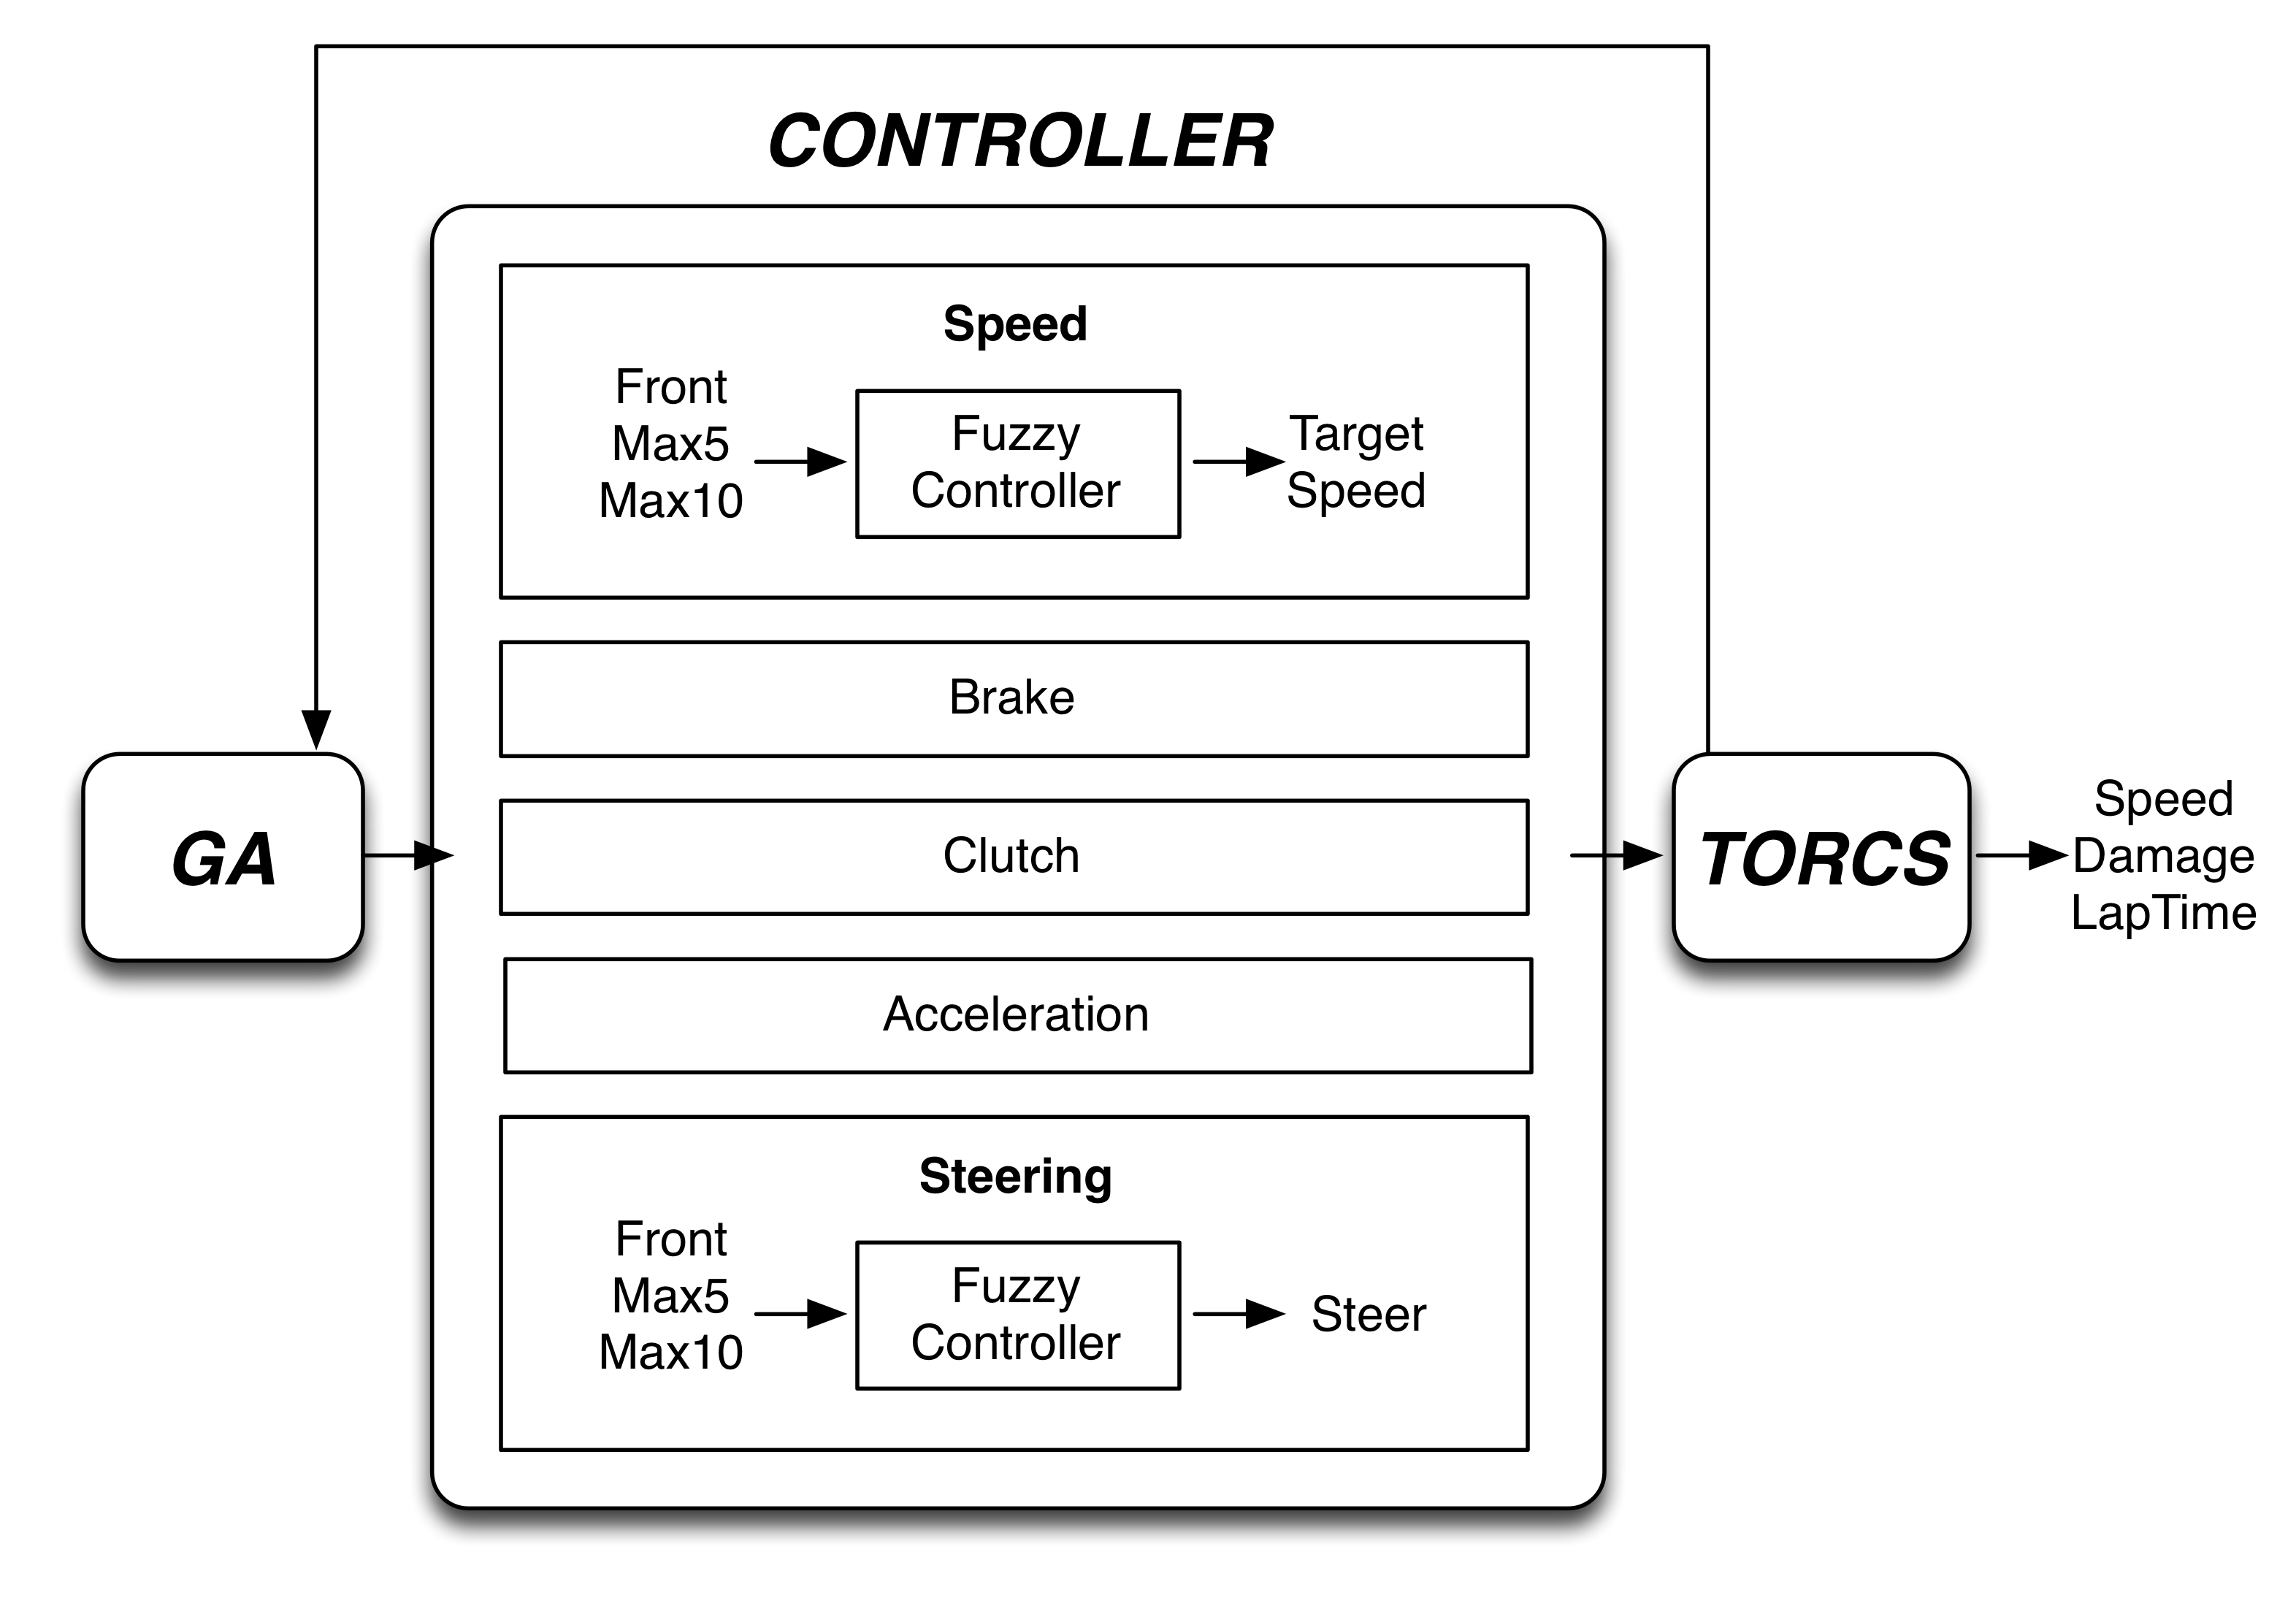
\includegraphics[width=9cm]{fig/flowchart}
 	\end{center}
 	\caption{Flowchart of the optimization process of a TORCS
          fuzzy controller. To evaluate an individual we put the
          parameter values of the two sub-controllers in the
          corresponding chromosome, then we launch a race in TORCS
          with this configuration, obtaining the resulting values of
          Average Speed and Damage. Individual's fitness value is
          computed using these values.} % This needs to be rewritten,
                                % since it's in the previous paper. - JJ
 \end{figure}

In our approach, every individual or chromosome is a vector of 18
values/parameters, 6 per variable (see Figure \ref {fig:cromosome}),
coded using real values aiming to have some precision
\cite{elsayed13}. 

 \begin{figure*}[!ht]	
 	\begin{center}
 		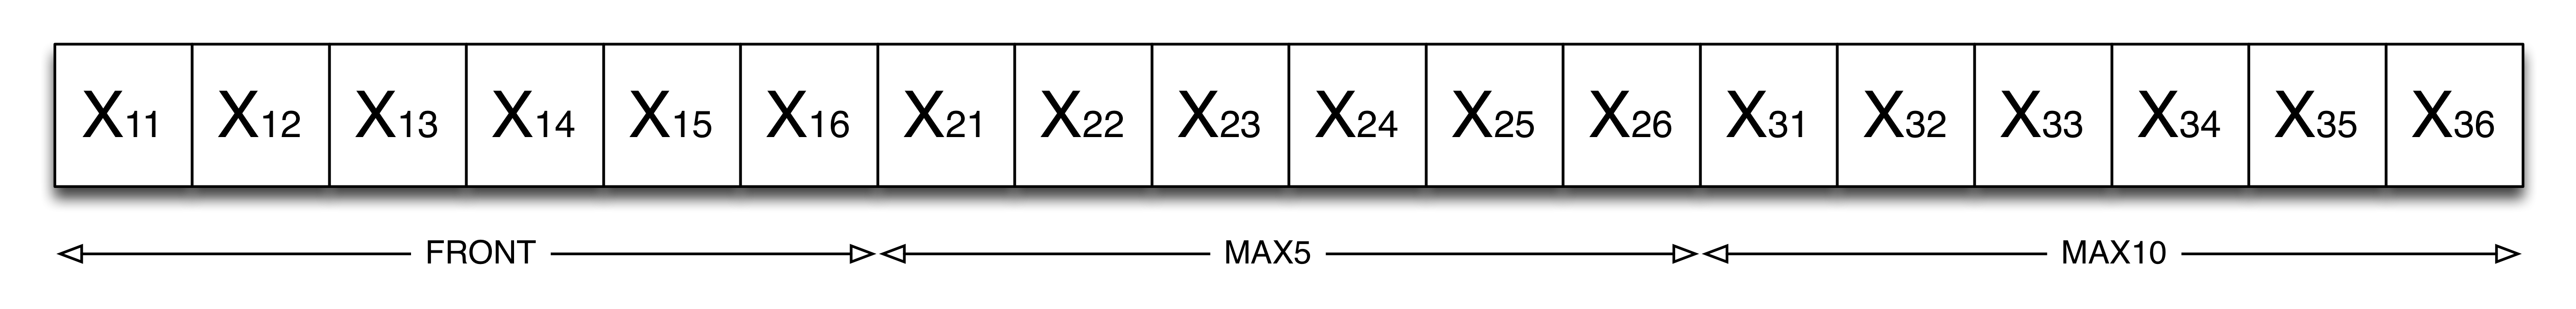
\includegraphics[width=10cm]{fig/chromosome2.png}
 		\caption{Chromosome description}
 		\label{fig:cromosome}	
 	\end{center}	
 \end{figure*}

Following standard implementations \cite{GAs_Goldberg89}, in the first step of the algorithm \cite{salem_evo17} a population of random individuals is composed by assigning diverse values inside a feasible range ($[0,100]$).

As it can be seen in Figure \ref{fig:ga}, TORCS is used for the
evaluation of every individual. This evaluation is based on different
fitness functions, which we have tested in previous works
\cite{salem_evo18}.  % This paragraph no longer applies, because in
                     % many cases we are using selection. It would be
                     % better to just rewrite the whole thing, taking
                     % into account the new GPS - JJ
However, in this study we will consider the function which obtained the best results in our previous paper \cite{salem_cig2018}, namely:

 \begin{equation} \label{fit2}
 	\begin{array}{lll}
 		f_{AVS}= \frac{AVG(Speed)}{Damage+1}
 	\end{array}
 \end{equation}	

Following the usual recommendations in the literature \cite{Harik-ParameterLess99}, we have defined a parameter-less function, where there are no weights in the terms.
At the same time, this fitness expression is closer to a `human-like' approach, given that it is focused on the real objectives for a controller during a race, rather than on the overall target of winning or not. 

It depends on two variables:

 \begin{itemize}
 	\item $AVG(Speed)$: pursues a combination of good driving in
          the difficult zones of the tracks (e.g. curves) and also on
          easy or straight parts; i.e. considers the overall behavior
          in the whole track. % needs to be rewritten. 
 	\item $Damage$: aims to create `safe' controllers, as it is
          mandatory being able to finish the race. % Also needs to be
                                % rewritten. 
 \end{itemize} 

 %% ----------------------- This needs to be rewritten since it's
 %% taken from another paper
So the function aims to obtain controllers reaching the highest average speed as possible on the whole track while avoiding damage to the vehicle.

As it is shown in Figure \ref{fig:ga}, the fitness of each candidate solution (individual) is computed by injecting its gene values to the parameters of the membership functions of the two fuzzy sub-controllers. Then, the defined autonomous controller drives a car in a 20 laps race in a circuit without opponents, and the obtained results (Average Speed and Damage) are used to compute the fitness value. 
Given that the objective of the car controller is to win as many races as
possible, we decided to optimize the most general case by carrying out solo {\em training races}, which will be less sensitive to the presence of \textit{noise/uncertainty} due to the participation of other controllers \cite{merelo2016statistical}.

In addition, we have considered the same track as in previous works
\cite{salem_cig2018} for this evaluation, because it has a proper
combination of curves and straight parts. This will aid to obtain an
`all-terrain behaviour' for the controllers.
% Up to here ----- JJ

Regarding the genetic operators, \textit{mutation} has remained the same as in previous approaches of our genetic controller, i.e. \textbf{non uniform mutation} \cite{mutation1997}. 

% We need to summarize this and refer to previous papers
% -------------------------

% Antonio - I have rewritten all this part. 
% Moreover, according to the invitation, this paper must be an extended version of the one published at CoG 2019, and I think it should contain a complete description of the main parts, as the Genetic algorithm proposed. I personally hate papers where you have to move to another 3 papers in order to understand the contents.


% Besides, this is also in the other paper - JJ ----------------------

% Antonio - Again, this must be an extended version and this is the main contribution. It should be here. I rewrite this.

This paper proposes the inclusion of two different mechanisms into the algorithm in order to improve its performance, as well as it allows to obtain better controllers overall.

The first technique is a \textbf{Grand Prix Selection policy} (GPS), which aims to select more reliable individuals/controllers to be parents of the following population, i.e. better deal with the uncertainty surrounding the election of an actual good individual. The mechanism arranges groups of 10 controllers (using the same car) and then different races of several laps are simulated in the same track of TORCS. After every race, the contenders obtain different scores depending on their position in the final rank. The best 5 controllers in the sum of all the races are selected as parents for the following generation. 

% Most of this paragraph needs to be rewritten - JJ
As it can be noticed, the application of this approach will be independent of the fitness value, so it can be considered as a \textit{fitness-less proposal}.
Thanks to this mechanism the best individuals will be more likely
selected to reproduce. Of course, it is not possible to assure they
are absolutely the best, due to the uncertainty present in this type
of environments, i.e. games against non-deterministic opponents
\cite{merelo2016statistical}. However, we argue that this selection
policy will be `less sensitive' to that uncertainty (or noise), and
thus, it will be fairer and more reliable than an approach purely
based on the fitness values.  

On the other hand, the application of this method consumes much higher computation time, so it could be combined with the classical fitness-based selection in some generations. Indeed, in the experiments conducted in Section \ref{sec:results}, we have analysed the impact of the application of different configurations of GPS, considering a different number of generations where to apply it.

The second technique implemented in our GA is the \textbf{BLX-$\alpha$ Crossover operator} \cite{blx2008}, which allows to control the balance between exploration and exploitation along the generations.

The Blend crossover operator starts by choosing randomly a number from the interval $[x_i-\alpha(y_i-x_i).. y_i+\alpha(y_i-x_i)]$, where $x_i$ and $y_i$ are the $i^{th}$ parameter values of the parent solutions $x$,$y$ and $x_i < y_i$. See Figure \ref{fig:blxalpha}.

 \begin{figure}[!ht]	
 	\begin{center}
 		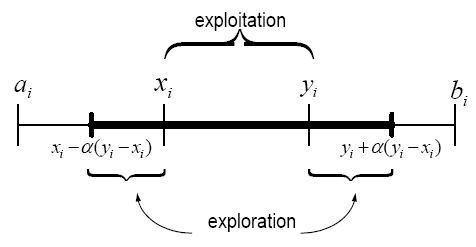
\includegraphics[width=5cm]{fig/blxalpha.jpg}
 		\caption{Blend crossover operator ($BLX-\alpha$)}
 		\label{fig:blxalpha}	
 	\end{center}	
 \end{figure}

 % Paragraphs to rewrite - JJ
Thus, this operator is based on the random generation of genes from the associated neighborhood of the genes in the parents. Three generated descendants are different among them and also among them and their parents, leading to a higher exploration factor in the generation of the offspring.
This operator is suitable for real coded genetic algorithms where it has proved to achieve a good balance between exploration and exploitation \cite{blx2008}.

$\alpha$ parameter allows to control the exploration of the space of solutions, depending on its value. So, in order to ensure the balance between exploitation and exploration of the search space, $\alpha = 0.5$ could be selected.

In GAs, the search process needs a high exploration rate in the first generations (high diversity) in order to explore multiple parts of the search space. But in the last generations, high exploitation is preferred to ensure the convergence to the optimal solution.

Given this, we have considered two different approaches in the experiments: one taking a constant value for $\alpha$, and another with a variable scheme, in which the value of $\alpha$ is decreased over the generations (getting sequentially more exploitation and less exploration). Thus, its value is obtained as:

 \begin{equation}
 	\label{eqalpha}
 	\alpha =1-\frac{g}{g_{max}}
 \end{equation}

Where $g$ is the current generation and $g_{max}$ is the maximum number of generations. We think that this approach can achieve an effective balance between exploitation and exploration and therefore, better solutions (better controllers) may be obtained.

% Up to here... - JJ
% All this is also from the other paper and does not really correspond
% to what we are doing in this paper - JJ
% Antonio - Yes, we have done the same here, but extending the
% experiments with other configurations for the GPS. ;)
% Needs to be rewritten anyway. - JJ

%%%%%%%%%%%%%%%%%%%%%%%%%%%%  RESULTS  %%%%%%%%%%%%%%%%%%%%%%%%%%%%

\section{Experiments and results}  
\label{sec:results}

% >>>>>> TODO: Explain the new experiments and results -> Mohammed  <<<<<<<<<<
% TODO: Results with GPS (no BLX-Alpha crossover)
% TODO: Results with GPS and BLX-Alpha crossover
% TODO: Comparison against the standard controllers in TORCS
% TODO: Comparison against S&PL controller (of all our controllers, if possible)

In this kind of problems, it is essential to select the correct
training track so that bots are able to work in a wide range of
conditions. Usually a single track, out of all the existing TORCS
ones, is selected, since evaluation in a single track takes some time
and using several of them would make evaluation too onerous. For
several papers already \cite{salem_cig2018,DBLP:conf/cig/SalemMG19},
we have been using the \textit{Alpine 2} track (See Figure
\ref{fig:alpine2_track}). This track has several characteristics that
are essential for evaluating a bot: it has got many turns, some of
them with 180 degrees, steep segments, and some very challenging parts
like the entrance of a tunnel at an square angle. All these features makes
it a good test bed for good turning and collision avoidance
strategies, but also a few straight segments which allow the car to
speed ahead, reaching high speeds. This same track has been repeatedly
used for training as well as for testing and has been described as
``technical and complex'' \cite{AG} and ``presenting a challenge even
at low speeds'' \cite{vrajitoru2018global}, for instance in
\cite{cardamone2010applying,CarRacing_Pelta09,zong2017obstacle}; in \cite{AG} it had
the third lowest lap time, after Alpine 1 and Olethros, implying it
has got a good balance between hardness and speed. Since we also used
it in our previous papers, it allowed us to compare racing bots that
had been ``trained'' in the same conditions.

\begin{figure}[!ht]	
	\begin{center}
		
\includegraphics[width=3cm]{fig/alpine2.jpg}
		\caption{Alpine 2 Track: Slow mountain road. Length: 3773.57m, Width: 10m}
		\label{fig:alpine2_track}	
	\end{center}	
\end{figure}

As in our others studies, we have used the vehicle \textit{car1-trb1},
which is a well balanced, NASCAR type car \footnote{See description in
  the TORCS racing board web page,
  \url{http://www.berniw.org/trb/cars/car_view.php?viewcarid=5}},
which we have used also in our previous papers, and also by many
winning bots along the history of the TORCS championship
\cite{torcs5} as well as other authors
\cite{auteur2010,li2019reinforcement}. This matches well the selection
of racing track, but being as it is a balanced car, allows driving to
fit itself to the controllers we are developing.

New Grand Prix Selection has been conducted considering \textit{Alpine 2} track, 5 races and 20 laps per race. 
We have defined a score function based in Formula 1 Grand prix schema, so the obtained punctuations depend on the car position in the final rank: 1 - 25 points, 2 - 18, 3 - 15, 4 - 12, 5 - 10, 6 - 8, 7 - 6, 8 - 4, 9 - 2, 10 - 1. The the starting grid (initial positions of cars) on these races was set randomly.\\

To analyze the influence of the new introduced Grand Prix Selection (GPS) and the crossover operator on the performance of the fuzzy controller, we have carried out  two main optimization processes based on the GPS: the first one uses the GPS with the two point crossover operator while the second uses the varying $BLX-\alpha$. \\
In the generations where the GPS is not used, the controllers are evaluated using the fitness function: $f_{AVS}$ (Equation \ref{fit2}).
We have run the algorithms with a population size of 60
individuals. The rest of parameters are: Generations=50, Crossover
rate=0.85, Mutation rate=0.09, and 10 different runs per
configuration. % this should probably go to a table, and also needs
               % some kind of justification. Does crossover rate
               % include BLX-alpha? - JJ
               % no 

In each process, three experimentations are performed, the GPS is
applied in every generation in the first experimentation, only in the
last generation the second and each 5 generations in the last one. % Rewrite this and use acronyms as defined above - JJ
 
When Grand Prix selection process is applied as in previous work \cite{salem_cig2018}, the individuals of the population compete in 5 races (of 5 laps) in the \textit{Alpine 2} track. The last 10 individuals  in the GPS selection are replaced with new ones in the next generation. The winner will be selected as the best controller of the run.

The evolution process was applied in separate groups of runs to obtain
the following controllers: % Clarify which ones have been used for the
                           % first time in this paper; make references
                           % to the rest - JJ
\begin{itemize}
	
	\item $GFC-GPSVAE$: A proposed controller obtained by applying $BLX-\alpha$ crossover operator with a varying value of $\alpha$ using Equation \ref{eqalpha} and GPS every generation. 
	\item $GFC-GPSE$: The proposed controller in this paper and obtained by applying the classical two points crossover operator (as in previous works) and GPS every generation. 
	
	\item $GFC-GPS5$: A controller obtained by applying the
          classical two points crossover operator (as in previous
          works) and GPS once every 5 generations and fitness
          $f_{AVS}$ in the others \cite{DBLP:conf/cig/SalemMG19}. % This was in a previous paper,
                                % please cite it - JJ
	\item $GFC-GPSL$: A controller obtained by applying the
          classical two points crossover operator (as in previous
          works) and GPS once in the last generation and fitness
          $f_{AVS}$ in the others\cite{DBLP:conf/cig/SalemMG19}. % This was in a previous paper - JJ

	\item $GFC-GPSVAL$: A controller obtained by applying $BLX-\alpha$ crossover operator with a varying value of $\alpha$ using Equation \ref{eqalpha} and GPS once in the last generation and fitness $f_{AVS}$ in the others\cite{DBLP:conf/cig/SalemMG19}. 

	\item $GFC-GPSVA5$: A controller obtained by applying $BLX-\alpha$ crossover operator with a varying value of $\alpha$ using Equation \ref{eqalpha} and GPS once every 5 generations and fitness $f_{AVS}$ in the others\cite{DBLP:conf/cig/SalemMG19}. 


        \item $GFC$: Controller  from our previous work \cite{salem_cig2018} with fitness  $f_{AVS}$ (Equation \ref{fit2}).
	\item $GFC-VA$: A controller obtained by applying $BLX-\alpha$
          crossover operator with a varying value of $\alpha$ using
          Equation \ref{eqalpha} and fitness $f_{AVS}$ \cite{DBLP:conf/cig/SalemMG19}.
         
          
               % wasn't this
                                % also in cig2018? - JJ
                                %% yes,  V is for varying alpha
\end{itemize}


\subsection{Uncertainty in fitness evaluation}

We need first to find out how different kind of selection procedures
affect uncertainty in scores. Better selection procedures should be
able to reduce it, making evolved controllers as centrally distributed
as possible; other kind of selections should keep distribution of
scores (for a single controller) skewed and lopsided; this is why we
have done an study of the distribution  of the genetic individuals of
three evolution processes $GFC$, $GFC-GPSE$ and $GFC-VAGPS5$. 


Skewness is related to how symmetric the distribution of fitness
scores is. There are several strategies that deal with this kind of
uncertain (usually called {\em noisy} fitness functions; but a simple
one is to re-evaluate ({\em re-sample}) the score every generation. A
skewed distribution mean that it will more likely to sample a value
that is different from the average, but it might be better or worse
than average; in any case, different from the score we would expect to
achieve in other circumstances. On the other hand, kurtosis measures
the amount of values that are far from the average, creating either a
heavy-tailed or too-lightly-tailed distribution. In the first case, it
will mean that values far from what would be expected are likely to
show up in the fitness score.

This is why we are interested in how these two statistical measures
are going to change with evolution; they will both affect
selectability of an individual, so that, in general, they will select
individuals with lower kurtosis and skewness, since they are more
likely to draw a consistent value and thus go ahead to the next
generation. However, different selection procedures will affect this
in different ways. This is why we have computed skewness and kurtosis for 1 in 5 individuals in the
population chosen randomly, and measured fitness values after the
first, the 20th and the last generation for the three controllers;
results are shown in Figures \ref{fig:gfcsk},\ref{fig:gfcrsesk} and
\ref{fig:gfcvarsesk}). % Which fitness score are we using? - JJ
%% Mohammed $f_{AVS}$ fitness for GFC and GPS for the others

\begin{figure}[!ht]	
	\begin{center}
		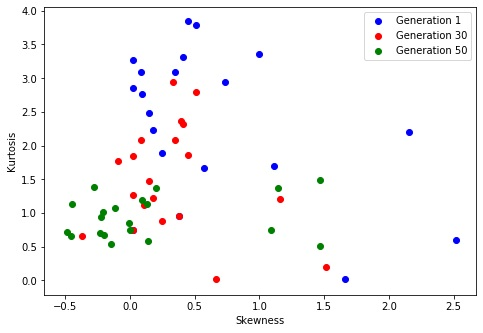
\includegraphics[width=9cm]{fig/GFC__.jpg}
		\caption{Skewness ($y$ axis) and kurtosis ($x$ axis)
                  for the fitness score in an experiment with the
                  $GFC$ method \cite{salem_cig2018}.}
		\label{fig:gfcsk}	
	\end{center}	
\end{figure}
\begin{figure}[!ht]	
	\begin{center}
		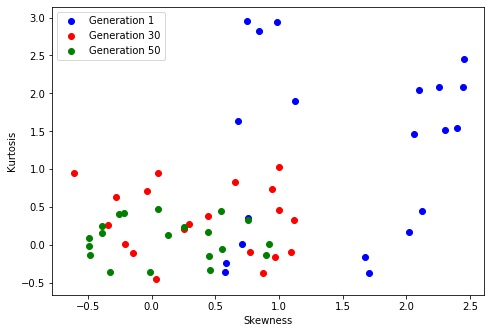
\includegraphics[width=9cm]{fig/GFCRSE__.jpg}
		\caption{Score skewness ($y$) and kurtosis ($x$) for
                  the fitless-ness method $GFC-GPSE$.}
		\label{fig:gfcrsesk}	
	\end{center}	
\end{figure}
\begin{figure}[!ht]	
	\begin{center}
		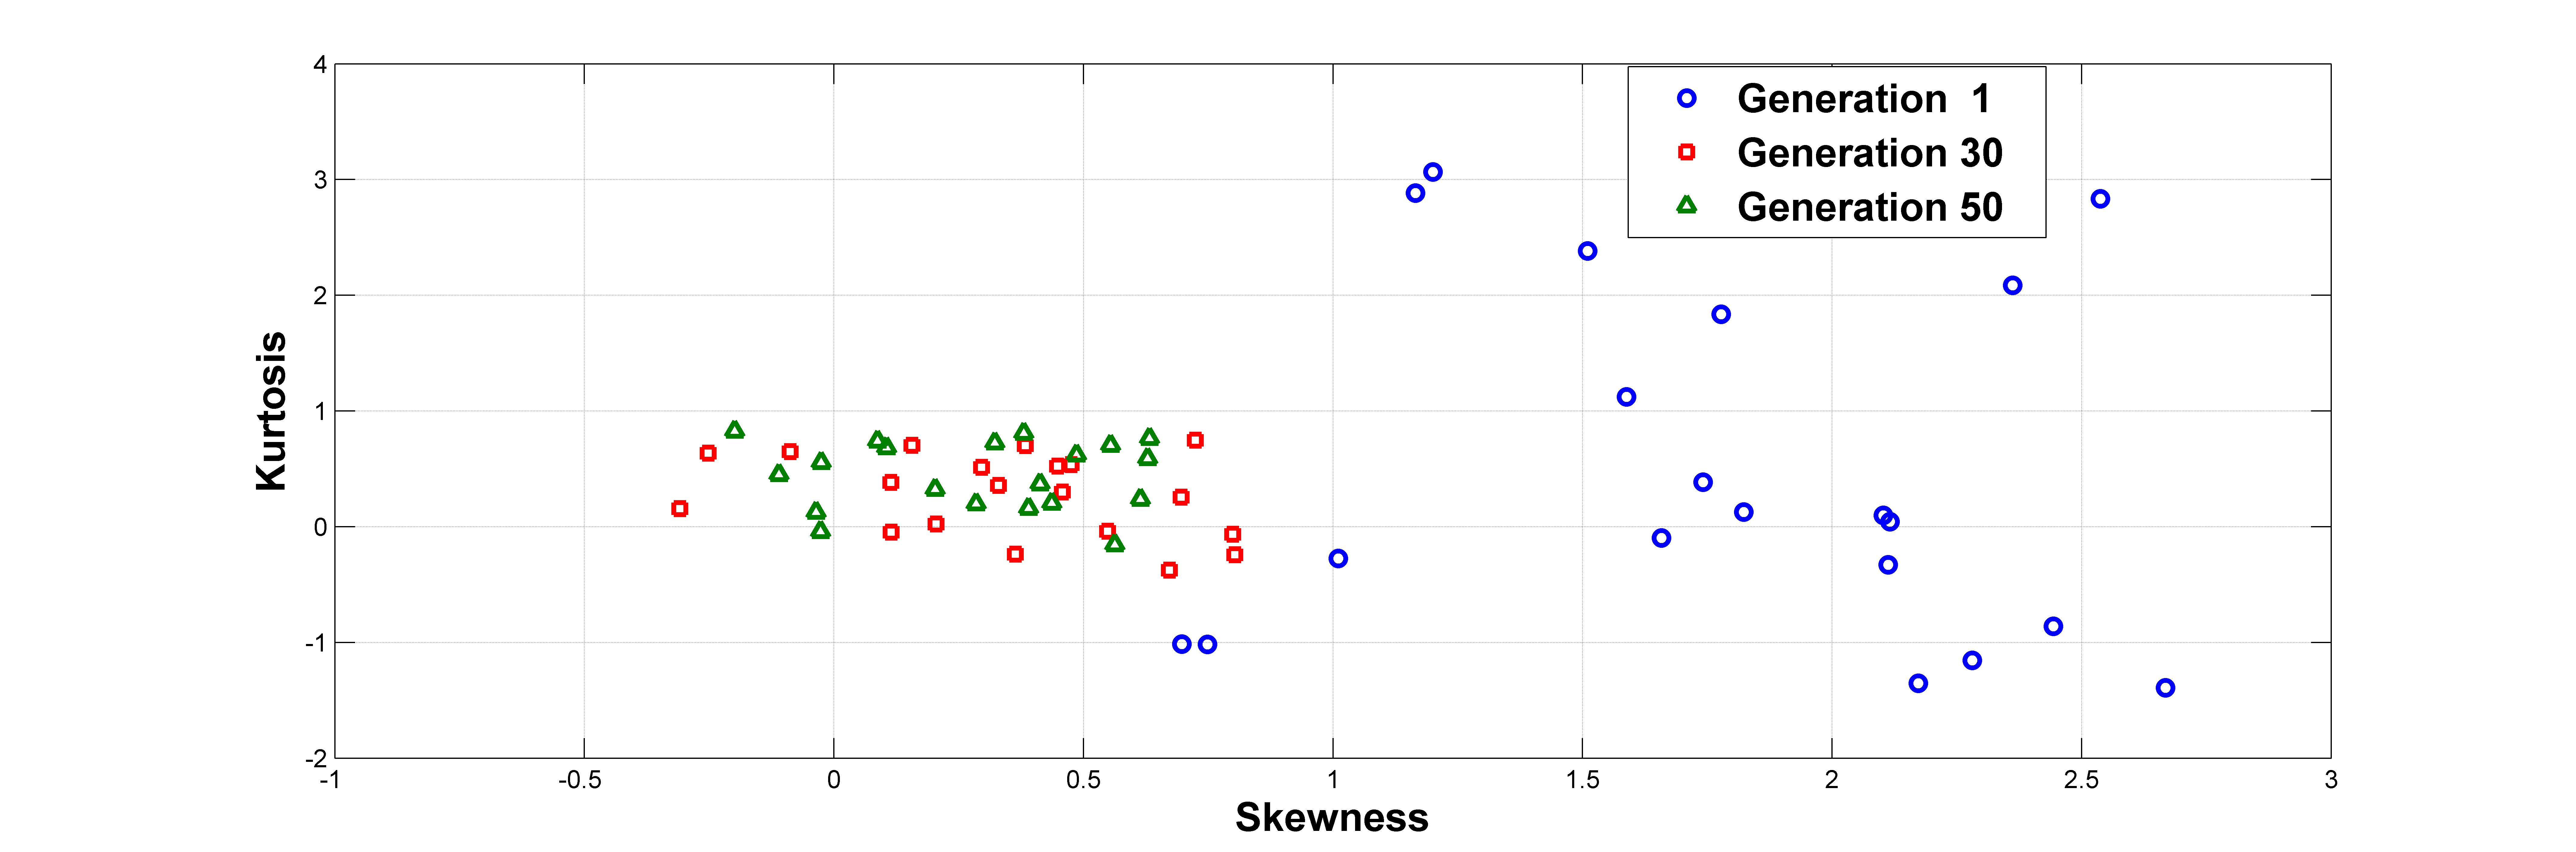
\includegraphics[width=9cm]{fig/GFCVARSE__.jpg}
		\caption{Skewness ($y$) and kurtosis ($x$) for
                  $GFC-VAGPSE$, which is fitless-ness and also uses
                  adaptive BLX$\alpha$ crossover.}
		\label{fig:gfcvarsesk}	
	\end{center}	
\end{figure}

All figures show that the evolution process has a certain influence in
these measures, with individuals in the latest stages of evolution
getting closer to the origin, which would be a 0-skewness, 0-kurtosis
Gaussian. However, there are differences between the fitness-based
process ({\sf GFC}) and the other two. In the first case, the
selection procedure simply eliminates the outliers with a high
skewness or kurtosis; there does not seem to be a big change from
generation 30 to 50, so as a matter of fact individuals with a high
and skewed variability are selected as {\em winners} when in fact they
are not.

The two fitless-ness methods, {\sf GFC-GPSE} and {\sf GFC−VAGPSE}, are
notably similar, with selection eventually concentrating individuals
close to a Gaussian distribution, although slighly skewed to the
right, and with a positive fat tail.

% Continue here -- JJ


% When comparing the three figures, a clear convergence, 
% is observed as generations pass but without reaching, the normal distribution; in the first
% generations, values of skewness and kurtosis are quite
% high and correspond to arbitrary uniform distribution, however, as the simulation proceeds, values
% approach zero. However, they do not converge
% exactly to 0, meaning that, even if uncertainty can be
% approached by a normal distribution, that approximation
% would only be correct for the latest generations\cite{noisylunch2015}.
% Another remarkable fact is the faster the convergence is in the case of $GFC-VAGPSE$ where it reaches its optimal values around the 20th generation to confirm the results of Table \ref{tab:time} where this controller evolution process has given the best individual between the eleventh and the eighteenth generation.
% This convergence speed is the result of the combination of $Alpha-BLX$ operator and the GPS which highly pressure the chromosomes.



\subsection{Testing Grand Prix selection and BLX-$\alpha$ controllers}


Once the 10 runs have finished, the obtained best controllers from the previous evolution processes compete again in a similar set of races, in order to choose the best controller overall per approach, i.e. the best between $GFC-GPSL$, $GFC-GPSE$ and $GFC-GPS5$, and between $GFC-GPSVAL$,$GFC-GPSVAE$ and $GFC-GPSVA5$.
Results are shown in Tables\ref{tab:RSresults} and \ref{tab:VaryingalphaRSresults}
%% Process 1 : GPS without Alpha
%% Process 2  : GPS with Alpha
%%  GFC and VA are used only in comparaison purpose

\begin{table*}[ht]
	\centering
	{\scriptsize
		\caption{ Results of $GFC-GPS$ controllers in a mini-championship with 10 controllers and 10
			races in two different tracks(20 laps each). {\tt tita}, {\tt berniw} and {\tt
				inferno} are example controllers included with the TORCS
			simulator \cite{torcs4}. We use {\bf boldface}
                      for the best value, {\em italics} for the second
                    best. }
		{
			\begin{tabular}{|c|c|c||c|}
				\hline
				controller&Score in \textit{Alpine 2} track &Score in \textit{E-Track 5} track &Total\\
				\hline
				\hline
				
			$GFC-GPS5$\cite{DBLP:conf/cig/SalemMG19}&	75	&74&	149\\
			$GFC-GPSE$&	98	&93&	{\bf 191}\\
			$GFC-GPSL$\cite{DBLP:conf/cig/SalemMG19}&	77	&81&	{\em 158}\\
			$GFC$ \cite{salem_cig2018}	&	56	&50&	106\\
			$GFC-VA$\cite{DBLP:conf/cig/SalemMG19}	&	46	&7&		53\\
			$inferno1$&	9	&8&		17\\
			$inferno2$&		20	&51&	71\\
			$berniw1$&	16	&24&	40\\
			$berniw2$&	76	&79&	155\\
			$tita1$&32	&38&	70\\		
				\hline
				
			\end{tabular}
		}\label{tab:RSresults}
	}
\end{table*}
%


%
\begin{table*}[ht]
	\centering
	{\scriptsize
		\caption{ Results of $GFC-VAGPS$ controllers in a mini-championship with 10 controllers and 10
			races in two different tracks(20 laps each). {\tt tita}, {\tt berniw} and {\tt
				inferno} are example controllers included with the TORCS
			simulator \cite{torcs4}. {\bf Boldface}
                      for the absolute winner, {\em italics} for the second
                    best.}
		{
			\begin{tabular}{|c|c|c||c|}
				\hline
				controller&Score in \textit{Alpine 2} track &Score in \textit{E-Track 5} track &Total\\
				\hline
				\hline	
				$GFC-VAGPS5$ \cite{DBLP:conf/cig/SalemMG19}&	82&	82&	{\em 164}\\
				$GFC-VAGPSE$&	108&    101&	{\bf 209}\\
				$GFC-VAGPSL$\cite{DBLP:conf/cig/SalemMG19}&	77&	73&	150\\
				$GFC$  \cite{salem_cig2018}&	56&	50&	106\\
				$GFC-VA$ \cite{DBLP:conf/cig/SalemMG19}&	46&	7&	53\\
				$inferno1$&	9&	8&	17\\
				$inferno2$&	20&	49&	69\\
				$berniw1$&	16&	24&	40\\
				$berniw2$&	59&	73&	132\\
				$tita1$&	32&	38&	70\\			
				\hline
				
			\end{tabular}
		}\label{tab:VaryingalphaRSresults}
	}
\end{table*}
%
As it could be noticed in the Table \ref{tab:RSresults}, the controller $GFC-VGPSAE$ has win the Grand Prix championship obtaining 98 points from 125 in the track used in the training, it has also ranked first in the track  \textit{E-Track 5}. //
The other GPS based controllers have obtained nearly the same results (149 and 158 respectively).
From Table \ref{tab:RSresults},it is clear that the controller $GFC-VAGPSE$, where GPS selection has been applied in every generation, has won the majority of possible points in the two previous tracks even the unknown \textit{E-Track 5}  track.

These results come to confirm the influence of the proposed selection policy where the controllers obtained from applying the GPS selection alone have won the competition.
 
This results is evident when comparing the points obtained by GPS controllers and GFC.
Indeed, we have made the selection process  realistic by eliminating
the classical fitness function based on the speed and damage average
and replacing it by points obtained in direct races. 
Better speed in solo racing is not a criterion of a good controller, the
best is the one who wins races. The new selection policy allows you to
select the winners on the field and not the possible winners. 
The following experimentation is dedicated to detect the impact of the $BLX-\alpha$.
The best controllers obtained from the two main optimization
processes: $GFC-VAGPSE$ and $GFC-GPSE$ are evaluated in formula like
championship against the references five TORCS bots and the $GFC-VA$\cite{DBLP:conf/cig/SalemMG19}
and $GFC$ controllers  \cite{salem_cig2018}. We have considered also an opponent from the
state of the art, which participated in several Simulated Car Racing
Competitions in past editions.  % Rewrite this paragraph too, from "We
                                % have considered" - JJ
It was proposed by P{\'e}rez-Li{\'e}bana, S{\'a}ez, Recio and Isasi \cite{EvolvingRuleSystem08} and later refined in the work \cite{PerezEvolvingFuzzy09}. We have baptised it as PSRI in honor of its authors' surnames.Results are in Table \ref{tab:allsresults}
%
\begin{table*}[ht]
	\centering
	{\scriptsize
		\caption{ Results of $GFC-GPSVAE$ and $GFC-GPSE$
                  controller in a mini-championship with 10 controllers
                  and 10 % you use driver here, controller
                         % elsewhere. Use always one or the other - JJ
                         %% mOhammed ok 
			races in two different tracks(20 laps each). {\tt tita}, {\tt berniw} and {\tt
				inferno} are example controllers included with the TORCS
			simulator \cite{torcs4}.  {\bf Boldface} is
                        used to highlight the best value, {\em italics} for the second
                    best.}
		{
			\begin{tabular}{|c|c|c||c|}
				\hline
				controller&Score in \textit{Alpine 2} track &Score in \textit{E-Track 5} track &Total\\
				\hline
				\hline
$GFC-GPSE$&	85&	82&	{\em 167}\\
$GFC-VAGPSE$&111&101&            {\bf 212}\\
$GFC$  \cite{salem_cig2018}&		48&	55&	103\\
$PSRI$\cite{PerezEvolvingFuzzy09}&		53&	48&	101\\
$GFC-VA$ \cite{DBLP:conf/cig/SalemMG19}&	78&	64&	142\\
$inferno1$&	9&	8&	17\\
$inferno2$&	20&	40&	60\\
$berniw1$&	16&	24&	40\\
$berniw2$&	59&	69&	128\\
$tita1$&	26&	18&	44\\
					\hline
				
			\end{tabular}
		}\label{tab:allsresults}
	}
\end{table*}
%



The above competition clearly demonstrates the superiority of the $GFC-VAGPSE$ controller where it clearly leads in the points. It collected most of the points in the two tracks, leaving the $GFC-GPSE$ controller far behind it. The reference conductors, namely $GFC-VA$ and $GFC$  are classified 3rd and 5th.
The introduction of the $BLX-\alpha$ operator allows the parameters of the controllers to be refined and  increases diversification in the optimization process, which has led to better results than those of $GFC-GPSE$.

To evaluate the cost of the proposed controllers, the table \ref{tab:time} shows the average number of laps % Isn't this
% average running time? - JJ
%% each lap in Alpine 2  takes between 90s and 120s
%%  I prefered the laps number to high time values ( 123800s for instance) 
and the range of the generation where the best individual is found of all the considered controllers. These results are obtained by running genetic
optimization for 50 generations for 10 runs.  

\begin{table}[!ht]
	\centering
	{\scriptsize
          \caption{Average number of laps per generation %  Isn't this
                                %  average running time? - JJ
            and
                  generation where the best individual was spawned.}
		\label{tab:time}
		\begin{tabular}{|p{2.85cm}|p{1.65cm}|p{1.65cm}|}
			\hline 	
			\hline  
			Controller& \textbf{Average Runtime}&\textbf{Generation}\\
% Is this number of laps or running time? - Jj
%Mohammed %% each lap in Alpine 2  takes between 90s and 120s
%% number of completed laps ,  I prefered the laps number to high values of average running time values ( 123800s for instance) 
                  \hline \textbf{\textbf{$GFC$}} \cite{salem_cig2018}&296 &34-39\\
			\hline \textbf{$GFC-VA$} \cite{DBLP:conf/cig/SalemMG19}&298	&10-18\\	
			\hline \textbf{$GFC-GPSL$} \cite{DBLP:conf/cig/SalemMG19}& 322&23-38\\	
			\hline \textbf{$GFC-GPS5$} \cite{DBLP:conf/cig/SalemMG19}&689	&24-38\\	
			\hline \textbf{$GFC-GPSE$}&	2488&22-40\\	
			\hline \textbf{$GFC-VAGPSL$} \cite{DBLP:conf/cig/SalemMG19}&321	&9-15\\	
			\hline\textbf{$GFC-VAGPS5$} \cite{DBLP:conf/cig/SalemMG19}&	691&8-17\\	
			\hline\textbf{$GFC-VAGPSE$}&2489	&11-18\\					
			\hline 
		\end{tabular}
		
	}
\end{table} 

The two $GFC-VAGPSE$ and $GFC-GPSE$ controllers were the best where they are ranked 1st and 2nd but they are very expensive in runtime where they have performed around 2490 laps in Alpine 2, which is a huge learning time.
The proposed selection policy is effective but in return requires a lot of time.

Another point that we can highlight is that the controllers with
$BLX-\alpha$ have reach the optimal solution in few generations
(between the 10th and the 20th) while the other methods required more
generations. 


 %%%%%%%%%%%%%%%%%%%%%%%%%%%%
\section{Conclusions and Future Work} 
\label{sec:conclusions}

% >>>>>> TODO: Rewrite this section -> All  <<<<<<<<<<


% In this paper we have tried to get winning racing car controllers by
% first improving the selection process so that, from time to time,
% uncertainty is eliminated by using actual competitions instead of
% fitness-based evolution, and second, keep the balance between
% exploration and exploitation high, and also variable, by using a fixed
% and adaptive version of the BLX-$\alpha$ operator.

% The fuzzy genetic controller is subject to uncertainties in the track especially in case of presence of rivals so in order to overcome this problem and thus design a robust and reliable bot, we proposed to apply a \textit{Grand Prix Selection policy} where the selection of parents in the evolutionary process is carried out according to the results of a set of mini-championships organized among the individuals of the population, which looks like a car racing tournament selection.
% At the same time, and aiming to intensify the exploration process in the search space, we used the $BLX-\alpha$ crossover operator with decreasing values of the $\alpha$ parameter throughout the generations.

% The evaluation was performed by comparing the proposed controller with bots of the TORCS platform, yielding very good results.
% The other evaluation of our controller was a confrontation with a real bot ($PSRI$ controller), which participated in several Simulated Car Racing Competitions. In this case, the BLX operator and the new selection policy have had a lot of impact in helping our controller to win three quarters of the races by getting the lowest damage, average speed and maximum speed values.

% These results let us to think that our controller could have reached a very good rank in the Simulated Car Racing Competition, which is unfortunately over since 2013. Anyway, we think that the findings of this study (and previous ones) could be applied successfully to other car racing simulators, such as those used in current eSports Competitions, such as iRace (https://www.iracing.com/).

% As future lines of work, this controller can be improved in some ways:
% We can extend the selection policy to all generations while overcoming the computation time drawback by means of a parallel implementation.
% We can also explore other parameter-less fitness functions to evaluate individuals including other factors affecting the performance of the car.
% Another perspective is to use multiple tracks (instead of just one) in the selection process in order to train a more general controller, able to deal with many different situations.

\section*{Acknowledgments}

This work has been supported in part by: Ministerio espa\~{n}ol de
Econom\'{\i}a y Competitividad under projects  TIN2017-85727-C4-2-P (UGR-DeepBio) and TEC2015-68752 (also funded by FEDER).

\bibliographystyle{IEEEtranS}
\bibliography{fuzzy_torcs,geneura,uncertainty}



\begin{IEEEbiographynophoto}{Juan~J.~Merelo}
Biography text here.
\end{IEEEbiographynophoto}

% You can push biographies down or up by placing
% a \vfill before or after them. The appropriate
% use of \vfill depends on what kind of text is
% on the last page and whether or not the columns
% are being equalized.

%\vfill

% Can be used to pull up biographies so that the bottom of the last one
% is flush with the other column.
%\enlargethispage{-5in}



% that's all folks
\end{document}


